%%%%%%%%%%%%%%%%%%%%%%%%%%%%%%%%%%%%%%%%%%%%%%%%%%%%%%%%%%%%%%%%%%%%%%%%%%%%%%%%

% IEEEconf.cls file must exist in the same directory as the TeX file you want to compile
\documentclass[letterpaper, 10 pt, conference]{IEEEconf}

\title{\LARGE \bf
COMPUTER HISTORY\\
\large Birth of a Computer
}

\author{Group Number 6\\
\small Gabriel Sullivan\\
\small Estevan Marquez\\
\small Pio Cunanan\\
}

% Image/graphics support
\usepackage{graphicx}
\graphicspath{ {./images/} }

% Formatting for lists
\usepackage{enumitem}

% Formatting for media
\usepackage{float}
\restylefloat{table}
\restylefloat{figure}

\begin{document}

\maketitle
\thispagestyle{empty}
\pagestyle{empty}


%%%%%%%%%%%%%%%%%%%%%%%%%%%%%%%%%%%%%%%%%%%%%%%%%%%%%%%%%%%%%%%%%%%%%%%%%%%%%%%%
\section*{ABSTRACT}
\textit{
Computers have changed the world. With information on any topic at the tip of our fingers, technology has boomed exponentially. We are in the Information Era.  
}

%%%%%%%%%%%%%%%%%%%%%%%%%%%%%%%%%%%%%%%%%%%%%%%%%%%%%%%%%%%%%%%%%%%%%%%%%%%%%%%%
\section{INTRODUCTION}

The birth of the computer, is absolutely fascinating. The computer makes human calculation 
speeds absolete. Expediting the engineering process. Humans can now plan tenfold as fast. 
AFter World War II the arms/space race had begun. The race to get man in space, during this 
time we didnt have the luxery of computers but we are on the cusp. We had human computers who 
would calculate by hand. Absolute geniuses, brains of the century. After we got man into 
space is when we first started getting to the use of computers. The once brains of the 
century are no obsolete and out of jobs. That one phrase shows the ability of computers. Now 
computers are in everyones home and everyone has litte computers in their pockets. We are in 
the Information Era.

%%%%%%%%%%%%%%%%%%%%%%%%%%%%%%%%%%%%%%%%%%%%%%%%%%%%%%%%%%%%%%%%%%%%%%%%%%%%%%%%
\section{TIME PERIOD}

As the demand for high amounts of computation rise, 
prototypes of machines that could makes these 
automatically surface. However, science has 
always struggled without to make any significant 
progress without money, but one avenue that as 
consistently made funds available has been war. 
Some of the earliest computers were employed of the 
battlefields of World War II, often used to help coordinate 
the massive number of troops involved in the struggles and 
keep these movements a secret from the enemy. Germany developed 
“Enigma Machines” (See Figure \ref{fig:EM}) to create ciphers that made 
intercepted messages almost impossible to decipher by hand, so to decipher 
these messages other countries made their own machines. With 
this many prototypes and more being created, each with 
similar purposes but different methods of fulfilling that purpose, 
the foundation for the creation for computers was laid.  
\begin{figure}[h!]
\centering
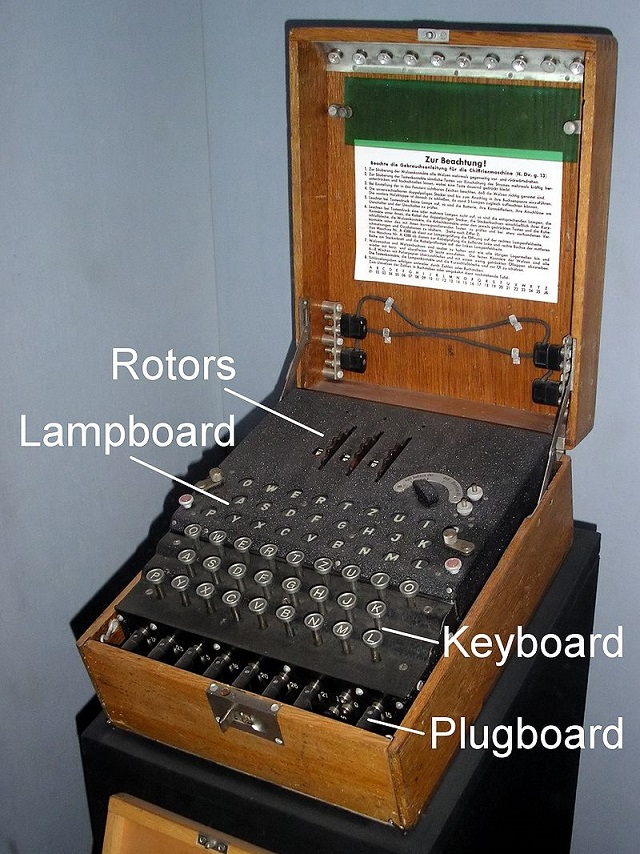
\includegraphics[width=0.5\textwidth]{EnigmaMachineLabeled}
\caption{A Recreated Enigma Machine}
\label{fig:EM}
\end{figure}   

%%%%%%%%%%%%%%%%%%%%%%%%%%%%%%%%%%%%%%%%%%%%%%%%%%%%%%%%%%%%%%%%%%%%%%%%%%%%%%%%
\section{COMPUTER HARDWARE}

You should list the specification of any hardware your topic
uses here. If you want make a table here, please label the table
and include discussion on what components are included in the
table and why. See Table
\ref{tbl:example} for an example of a table.
The labels/captions of the table should be put at the bottom
of the table.


\begin{table}[h!]
\begin{center}
\begin{tabular}{||c | c | c | c||} 
\hline
  & Col1 & Col2 & Col3 \\ [0.5ex]
\hline\hline
Row1 & (1,1) & (1,2) & (1,3) \\ 
\hline
Row2 & (2,1) & (2,2) & (2,3) \\
\hline
Row3 & (3,1) & (3,2) & (3,3) \\
\hline
\end{tabular}
\caption{Example of a table}
\label{tbl:example}
\end{center}
\end{table}

You might want to put figures in the document. Please
remember to label them. The labels/captions of the figures
should be put at the bottom of the figure. See Figure
\ref{fig:example} for an example of how to use figures.
You will need to place the figure in an \texttt{images/} folder
in your working directory.

\begin{figure}[h!]
\centering
\includegraphics[width=0.5\textwidth]{spiral.png}
\caption{Example of a figure}
\label{fig:example}
\end{figure} 

\section{COMPUTER SOFTWARE}
Since the requirements of these early computers were 
awfully specific, they did not have software developed 
for them, and the instructions that a computer would follow 
was purely dependent on its mechanical features. 
This changed with Manchester Mark I, which featured the 
very first stored program, giving rise to the development 
of software. By creating instructions in the form of computer 
memory, multiple processes could be performed by a single 
computer, and those processes could become even more complex 
with a fraction of the setup time.

\section{CONCLUSION}

Conclude your research paper with any reflections on what you
learned about your topic. Was this what you expected to find?
Did you find any facts that surprised you? You may add other
personal reflections about the topic here.

\section*{REFERENCES}

Below are basic formats for different types of references.

\begin{enumerate}[label={[\arabic*]}]
\item Name of Author, ``Title of chapter in the book,''
Title of The Published Book, xth edition. City of
Publisher, Country if not U.S.
\item Name of Author, “Name of paper,” Abbrev.
Title of Periodical, vol. x, no. x, pp. xxx-xxx,
Abbrev. Month, year.
\item Name of Author, (Year, Month),
Title of Internet Article [Online]. Available E-Mail:
E-Mail.
\item Martin Campbell-Kelly, John Gustafson, 
Brian Randall, Horst Zuse, (2011, January),
Revolution [Online]. Available E-Mail:
For E-mail, see https://computerhistory.org/contact-us/.
\end{enumerate}

\end{document}
